\documentclass{beamer}

% TikZ = desen vectorial direct in LaTeX.
\usepackage{tikz}

% PGFPlots = grafice 2D/3D peste TikZ.
\usepackage{pgfplots}

\pgfplotsset{compat=1.18}

\begin{document}

% -----------------------------------------------------------------
% EXEMPLU 1: Suprafata 3D din coordonate discrete.
% CUM:
%   - furnizam puncte (x,y,z) explicit prin coordinates
%   - PGFPlots trianguleaza/interpoleaza pentru surf
% -----------------------------------------------------------------
\begin{frame}{Example 1 - basic coordinate surface plot}
  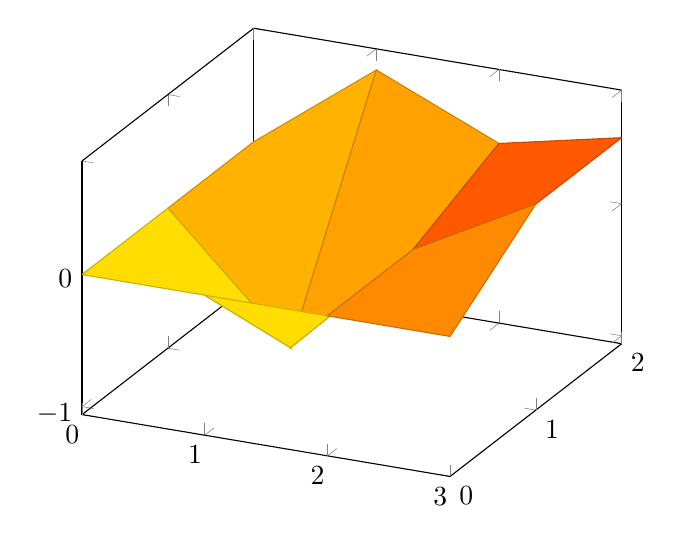
\begin{tikzpicture}
    \begin{axis}
      %From the PGFPlots manual.
      \addplot3 [surf] coordinates {
        (0,0,0) (1,0,0)   (2,0,0)   (3,0,0)
        
        (0,1,0) (1,1,-0.9) (2,1,0.0) (3,1,0.5)
 
        (0,2,0) (1,2,0.7) (2,2,0.3) (3,2,0.5)
      };
    \end{axis} 
  \end{tikzpicture}
\end{frame}

% -----------------------------------------------------------------
% EXEMPLU 2.1: Suprafata z = x^2 + y^2 calculata direct de PGFPlots.
% Observatie: randarea 3D poate fi mai lenta in pdflatex.
% -----------------------------------------------------------------
\begin{frame}{Example 2-basic, try using lualatex}
  %3D plots might be slow in the pasic pdflatex engine.
  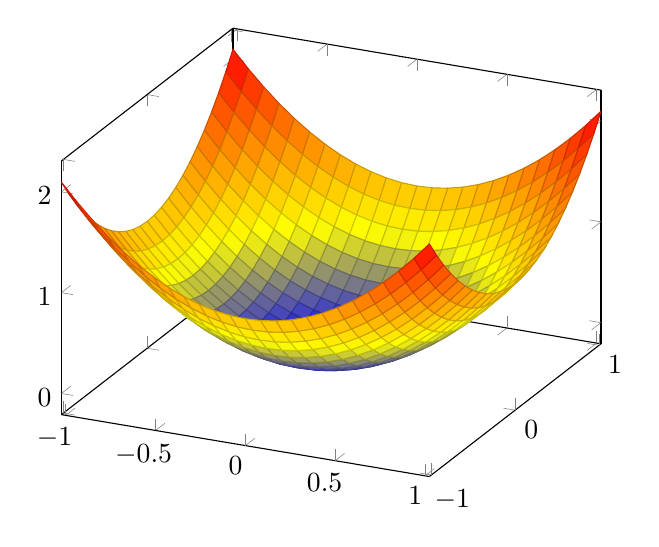
\begin{tikzpicture}
    \begin{axis}
      \addplot3+ [domain=-1.024:1.024,surf,no marks] {x * x + y * y};
    \end{axis}
  \end{tikzpicture}
\end{frame}

% -----------------------------------------------------------------
% EXEMPLU 2.2: Aceeasi suprafata, evaluata cu gnuplot extern.
% Necesita shell-escape / write18 pentru apel extern.
% -----------------------------------------------------------------
\begin{frame}{Example 2-gnuplot, try using shell-escape}
  %Look up shell-escape or write18 to be able to run this. 
  \begin{tikzpicture}
    \begin{axis}
      \addplot3+ [domain=-1.024:1.024,surf,no marks]  gnuplot {x * x + y * y};
    \end{axis}
  \end{tikzpicture}
\end{frame}

% -----------------------------------------------------------------
% EXEMPLU 3: Variatie vizuala prin colormap + shader interpolat.
% -----------------------------------------------------------------
\begin{frame}{Example 3, different colouring}
  %colormap/cool gives the blue colouring
  %shader=interp interpolates every pixel.
  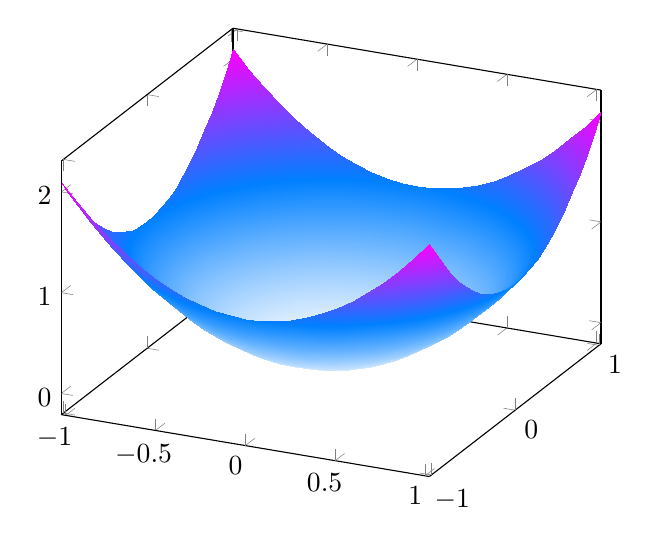
\begin{tikzpicture}
    \begin{axis}[colormap/cool]
      \addplot3+ [domain=-1.024:1.024,surf,no marks,shader=interp] {x * x + y * y};
    \end{axis}
  \end{tikzpicture}
\end{frame}

% -----------------------------------------------------------------
% EXEMPLU 4: Contururi 3D + proiectie pe plan z constant.
% CUM:
%   - primul plot: contururi pe suprafata
%   - al doilea plot: aceleasi contururi proiectate la z=-1
% -----------------------------------------------------------------
\begin{frame}{Example 4, contour gnuplot and projection}
  %A contour gnuplot is a 3D contour plot which requires gnuplot to compute it.
  \begin{tikzpicture}
    \begin{axis}[colormap/cool]
      \addplot3+ [
        domain=-1.024:1.024,
        no marks,
        contour gnuplot={
          number=20, %how many contours
          labels=false
        }
      ]
       {x * x + y * y};
      \addplot3+ [
        domain=-1.024:1.024,
        no marks,
        contour gnuplot={
          number=20,
          labels=false,
          %otherwise the z filter will not work:
          %give each point metadata its raw z value,
          %so we can filter it below
          output point meta=rawz,
        },
        %force the z-value to a constant, so we can project the plot.
        z filter/.code={\def\pgfmathresult{-1}} 
      ]
                 {x * x + y * y};

    \end{axis}
  \end{tikzpicture}
\end{frame}

% -----------------------------------------------------------------
% EXEMPLU 5: Suprapunere proiectie de contur + suprafata completa.
% -----------------------------------------------------------------
\begin{frame}{Example 5, plot and projection}
  \begin{tikzpicture}
    \begin{axis}[colormap/cool]
      \addplot3+ [
        domain=-1.024:1.024,
        no marks,
        contour gnuplot={
          number=20,
          labels=false,
          output point meta=rawz,
        },
        z filter/.code={\def\pgfmathresult{-1}}
      ]
                 {x * x + y * y};

      \addplot3+ [
        domain=-1.024:1.024,
        no marks,
        surf
      ]
      gnuplot {x * x + y * y};
    \end{axis}
  \end{tikzpicture}
\end{frame}

% -----------------------------------------------------------------
% EXEMPLU 6: Scatterplot 3D simplu din iris.csv.
% CUM:
%   - mapam axele pe sepal_length, sepal_width, petal_length
%   - afisam toate punctele cu acelasi marker
% -----------------------------------------------------------------
\begin{frame}{Example 6}
  \begin{tikzpicture}
    \begin{axis} [
        title={Subspecies separation},
        xlabel=Sepal length,
        ylabel=Sepal width,
        zlabel=Petal length,
        %legend, %would get in the way at default settings
        legend style ={anchor=north west, align=left},
        view={-30}{30},%rotate the axis
      ]
      \addplot3[only marks, mark=o,draw=red] table[col sep=comma,x=sepal_length,y=sepal_width,z=petal_length]{iris.csv};
      \addlegendentry{Everything};
    \end{axis} 
  \end{tikzpicture}
\end{frame}

% -----------------------------------------------------------------
% TASK 1: Suprafata functiei Rastrigin in 3D.
% Formula:
%   f(x,y)=20 + x^2 - 10*cos(2*pi*x) + y^2 - 10*cos(2*pi*y)
% CUM:
%   - domeniu standard [-5.12, 5.12] pe ambele axe
%   - esantionare pe grila pentru suprafata continua
% -----------------------------------------------------------------
\begin{frame}{Task 1: Rastrigin's function - like this}
  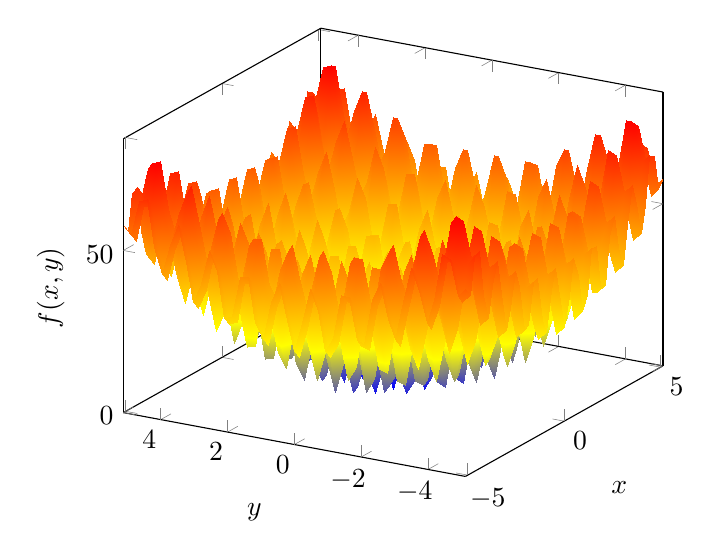
\begin{tikzpicture}
    \begin{axis}[
      view={-60}{25},
      domain=-5.12:5.12,
      y domain=-5.12:5.12,
      samples=45,
      samples y=45,
      xlabel={$x$},
      ylabel={$y$},
      zlabel={$f(x,y)$},
      colormap/hot,
      zmin=0,
    ]
      \addplot3[surf,shader=interp]
        {20 + x^2 - 10*cos(deg(2*pi*x)) + y^2 - 10*cos(deg(2*pi*y))};
    \end{axis}
  \end{tikzpicture}
\end{frame}

% -----------------------------------------------------------------
% TASK 2: Scatterplot 3D pe clase (Setosa/Versicolor/Virginica).
% CUM:
%   - filtram fiecare specie cu restrict expr to domain
%   - folosim marker diferit pentru separare vizuala
% -----------------------------------------------------------------
\begin{frame}{Task 2: 3D scatterplot}
  \begin{tikzpicture}
    \begin{axis}[
      title={Subspecies separation},
      xlabel=Sepal length,
      ylabel=Sepal width,
      zlabel=Petal length,
      xmin=4.3,
      xmax=7.9,
      ymin=2.0,
      ymax=4.6,
      zmin=0.8,
      zmax=7.0,
      xtick={5,6,7},
      ytick={2,3,4},
      ztick={5},
      width=9.6cm,
      height=6.3cm,
      legend style={anchor=north west, at={(0.86,0.84)}, align=left, draw=black, fill=white},
      view={-120}{23},
    ]
      \addplot3[
        only marks,
        mark=o,
        mark size=1.8pt,
        mark options={draw=red, fill=white, line width=0.5pt}
      ] table[
        col sep=comma,
        x=sepal_length,
        y=sepal_width,
        z=petal_length,
        restrict expr to domain={\thisrow{species_id}}{0:0}
      ]{iris.csv};
      \addlegendentry{Setosa}

      \addplot3[
        only marks,
        mark=triangle,
        mark size=2.0pt,
        mark options={draw=green!70!black, fill=white, line width=0.5pt}
      ] table[
        col sep=comma,
        x=sepal_length,
        y=sepal_width,
        z=petal_length,
        restrict expr to domain={\thisrow{species_id}}{1:1}
      ]{iris.csv};
      \addlegendentry{Versicolor}

      \addplot3[
        only marks,
        mark=diamond,
        mark size=1.8pt,
        mark options={draw=blue, fill=white, line width=0.5pt}
      ] table[
        col sep=comma,
        x=sepal_length,
        y=sepal_width,
        z=petal_length,
        restrict expr to domain={\thisrow{species_id}}{2:2}
      ]{iris.csv};
      \addlegendentry{Virginica}
    \end{axis}
  \end{tikzpicture}
\end{frame}

% -----------------------------------------------------------------
% TASK 3: Explicatie vizuala pe scatterplot (layer + codare culoare).
% CUM:
%   - adaugam un plan de referinta la petal length ~ 2.45
%   - coloram punctele dupa petal_width (point meta)
% -----------------------------------------------------------------
\begin{frame}{Task 3: Explanation on scatterplot}
  \begin{tikzpicture}
    \begin{axis}[
      title={Subspecies separation + petal width encoding},
      xlabel=Sepal length,
      ylabel=Sepal width,
      zlabel=Petal length,
      xmin=4.3,
      xmax=8.0,
      ymin=2.0,
      ymax=4.6,
      zmin=0.8,
      zmax=7.0,
      xtick={5,6,7,8},
      ytick={2,3,4},
      ztick={5},
      width=9.8cm,
      height=6.4cm,
      view={-35}{26},
      legend style={
        anchor=north west,
        at={(0.60,0.82)},
        align=left,
        draw=black,
        fill=white,
        font=\small,
        /tikz/text width=5.2cm
      },
      colormap/viridis,
      point meta min=0.1,
      point meta max=2.6,
    ]
      \addplot3[
        surf,
        shader=flat,
        draw=none,
        fill=orange,
        fill opacity=0.12,
        samples=2,
        domain=4.3:8.0,
        y domain=2.0:4.5,
      ] ({x},{y},{2.45});
      \addlegendentry{Plane: petal length \approx 2.45}

      \addplot3[
        only marks,
        scatter,
        mark=o,
        mark size=1.4pt,
        scatter src=explicit,
      ] table[
        col sep=comma,
        x=sepal_length,
        y=sepal_width,
        z=petal_length,
        meta=petal_width,
      ]{iris.csv};
      \addlegendentry{All samples\\(colour = petal width)}
    \end{axis}
  \end{tikzpicture}
\end{frame}

\end{document}
